\documentclass[11pt,preprint, authoryear]{elsarticle}

\usepackage{lmodern}
%%%% My spacing
\usepackage{setspace}
\setstretch{1.2}
\DeclareMathSizes{12}{14}{10}{10}

% Wrap around which gives all figures included the [H] command, or places it "here". This can be tedious to code in Rmarkdown.
\usepackage{float}
\let\origfigure\figure
\let\endorigfigure\endfigure
\renewenvironment{figure}[1][2] {
    \expandafter\origfigure\expandafter[H]
} {
    \endorigfigure
}

\let\origtable\table
\let\endorigtable\endtable
\renewenvironment{table}[1][2] {
    \expandafter\origtable\expandafter[H]
} {
    \endorigtable
}


\usepackage{ifxetex,ifluatex}
\usepackage{fixltx2e} % provides \textsubscript
\ifnum 0\ifxetex 1\fi\ifluatex 1\fi=0 % if pdftex
  \usepackage[T1]{fontenc}
  \usepackage[utf8]{inputenc}
\else % if luatex or xelatex
  \ifxetex
    \usepackage{mathspec}
    \usepackage{xltxtra,xunicode}
  \else
    \usepackage{fontspec}
  \fi
  \defaultfontfeatures{Mapping=tex-text,Scale=MatchLowercase}
  \newcommand{\euro}{€}
\fi

\usepackage{amssymb, amsmath, amsthm, amsfonts}

\def\bibsection{\section*{References}} %%% Make "References" appear before bibliography


\usepackage[round]{natbib}

\usepackage{longtable}
\usepackage[margin=2.3cm,bottom=2cm,top=2.5cm, includefoot]{geometry}
\usepackage{fancyhdr}
\usepackage[bottom, hang, flushmargin]{footmisc}
\usepackage{graphicx}
\numberwithin{equation}{section}
\numberwithin{figure}{section}
\numberwithin{table}{section}
\setlength{\parindent}{0cm}
\setlength{\parskip}{1.3ex plus 0.5ex minus 0.3ex}
\usepackage{textcomp}
\renewcommand{\headrulewidth}{0.2pt}
\renewcommand{\footrulewidth}{0.3pt}

\usepackage{array}
\newcolumntype{x}[1]{>{\centering\arraybackslash\hspace{0pt}}p{#1}}

%%%%  Remove the "preprint submitted to" part. Don't worry about this either, it just looks better without it:
\makeatletter
\def\ps@pprintTitle{%
  \let\@oddhead\@empty
  \let\@evenhead\@empty
  \let\@oddfoot\@empty
  \let\@evenfoot\@oddfoot
}
\makeatother

 \def\tightlist{} % This allows for subbullets!

\usepackage{hyperref}
\hypersetup{breaklinks=true,
            bookmarks=true,
            colorlinks=true,
            citecolor=blue,
            urlcolor=blue,
            linkcolor=blue,
            pdfborder={0 0 0}}


% The following packages allow huxtable to work:
\usepackage{siunitx}
\usepackage{multirow}
\usepackage{hhline}
\usepackage{calc}
\usepackage{tabularx}
\usepackage{booktabs}
\usepackage{caption}


\newenvironment{columns}[1][]{}{}

\newenvironment{column}[1]{\begin{minipage}{#1}\ignorespaces}{%
\end{minipage}
\ifhmode\unskip\fi
\aftergroup\useignorespacesandallpars}

\def\useignorespacesandallpars#1\ignorespaces\fi{%
#1\fi\ignorespacesandallpars}

\makeatletter
\def\ignorespacesandallpars{%
  \@ifnextchar\par
    {\expandafter\ignorespacesandallpars\@gobble}%
    {}%
}
\makeatother

\newlength{\cslhangindent}
\setlength{\cslhangindent}{1.5em}
\newenvironment{CSLReferences}%
  {\setlength{\parindent}{0pt}%
  \everypar{\setlength{\hangindent}{\cslhangindent}}\ignorespaces}%
  {\par}


\urlstyle{same}  % don't use monospace font for urls
\setlength{\parindent}{0pt}
\setlength{\parskip}{6pt plus 2pt minus 1pt}
\setlength{\emergencystretch}{3em}  % prevent overfull lines
\setcounter{secnumdepth}{5}

%%% Use protect on footnotes to avoid problems with footnotes in titles
\let\rmarkdownfootnote\footnote%
\def\footnote{\protect\rmarkdownfootnote}
\IfFileExists{upquote.sty}{\usepackage{upquote}}{}

%%% Include extra packages specified by user
\usepackage{booktabs}
\usepackage{longtable}
\usepackage{array}
\usepackage{multirow}
\usepackage{wrapfig}
\usepackage{float}
\usepackage{colortbl}
\usepackage{pdflscape}
\usepackage{tabu}
\usepackage{threeparttable}
\usepackage{threeparttablex}
\usepackage[normalem]{ulem}
\usepackage{makecell}
\usepackage{xcolor}

%%% Hard setting column skips for reports - this ensures greater consistency and control over the length settings in the document.
%% page layout
%% paragraphs
\setlength{\baselineskip}{12pt plus 0pt minus 0pt}
\setlength{\parskip}{12pt plus 0pt minus 0pt}
\setlength{\parindent}{0pt plus 0pt minus 0pt}
%% floats
\setlength{\floatsep}{12pt plus 0 pt minus 0pt}
\setlength{\textfloatsep}{20pt plus 0pt minus 0pt}
\setlength{\intextsep}{14pt plus 0pt minus 0pt}
\setlength{\dbltextfloatsep}{20pt plus 0pt minus 0pt}
\setlength{\dblfloatsep}{14pt plus 0pt minus 0pt}
%% maths
\setlength{\abovedisplayskip}{12pt plus 0pt minus 0pt}
\setlength{\belowdisplayskip}{12pt plus 0pt minus 0pt}
%% lists
\setlength{\topsep}{10pt plus 0pt minus 0pt}
\setlength{\partopsep}{3pt plus 0pt minus 0pt}
\setlength{\itemsep}{5pt plus 0pt minus 0pt}
\setlength{\labelsep}{8mm plus 0mm minus 0mm}
\setlength{\parsep}{\the\parskip}
\setlength{\listparindent}{\the\parindent}
%% verbatim
\setlength{\fboxsep}{5pt plus 0pt minus 0pt}



\begin{document}



\begin{frontmatter}  %

\title{The Impact of Loadshedding on SWIX sectors using DCC-GARCH
models}

% Set to FALSE if wanting to remove title (for submission)




\author[Add1]{Sven Wellmann}
\ead{20850980@sun.ac.za}





\address[Add1]{Stellenbosch University, Stellenbosch, South Africa}


\begin{abstract}
\small{
Abstract
}
\end{abstract}

\vspace{1cm}





\vspace{0.5cm}

\end{frontmatter}



%________________________
% Header and Footers
%%%%%%%%%%%%%%%%%%%%%%%%%%%%%%%%%
\pagestyle{fancy}
\chead{}
\rhead{}
\lfoot{}
\rfoot{\footnotesize Page \thepage}
\lhead{}
%\rfoot{\footnotesize Page \thepage } % "e.g. Page 2"
\cfoot{}

%\setlength\headheight{30pt}
%%%%%%%%%%%%%%%%%%%%%%%%%%%%%%%%%
%________________________

\headsep 35pt % So that header does not go over title




\hypertarget{introduction}{%
\section{\texorpdfstring{Introduction
\label{Introduction}}{Introduction }}\label{introduction}}

\hypertarget{data}{%
\section*{Data}\label{data}}
\addcontentsline{toc}{section}{Data}

\begin{figure}[H]

{\centering \includegraphics{Paper_files/figure-latex/CumRet-1} 

}

\caption{Cumulative Returns per Sector for ALSI and SWIX \label{CumRet}}\label{fig:CumRet}
\end{figure}

\begin{figure}[H]

{\centering 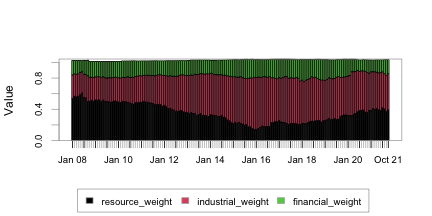
\includegraphics{Paper_files/figure-latex/ALSI-1} 

}

\caption{ALSI Weight Contribution \label{ALSI}}\label{fig:ALSI}
\end{figure}

\begin{figure}[H]

{\centering 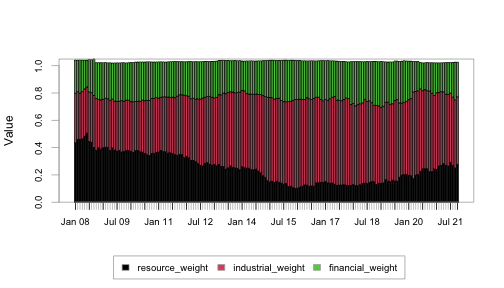
\includegraphics{Paper_files/figure-latex/SWIX-1} 

}

\caption{SWIX Weight Contribution \label{SWIX}}\label{fig:SWIX}
\end{figure}

\begin{figure}[H]

{\centering \includegraphics{Paper_files/figure-latex/LogRet-1} 

}

\caption{Log Returns per Sector for the SWIX \label{LogRet}}\label{fig:LogRet}
\end{figure}

\hypertarget{dcc-garch-model-fit}{%
\section{DCC GARCH Model Fit}\label{dcc-garch-model-fit}}

\hypertarget{estimate-std.-error-t-value-pr-t}{%
\subsection{Estimate Std. Error t value Pr(\textgreater{} \textbar{}
t\textbar{} )}\label{estimate-std.-error-t-value-pr-t}}

{[}Resources{]}.omega 0.00000 0.00001 0.304 0.761\\
{[}Resources{]}.alpha1 0.005 0.033 0.147 0.883\\
{[}Resources{]}.beta1 0.947 0.050 18.750 0\\
{[}Industrials{]}.omega 0.00000 0.00000 1.755 0.079\\
{[}Industrials{]}.alpha1 0.017 0.009 1.822 0.068\\
{[}Industrials{]}.beta1 0.907 0.017 54.781 0\\
{[}Financials{]}.omega 0.00000 0.00000 0.966 0.334\\
{[}Financials{]}.alpha1 0.032 0.022 1.492 0.136\\
{[}Financials{]}.beta1 0.907 0.033 27.601 0\\
{[}Joint{]}dcca1 0.039 0.005 7.807 0\\
{[}Joint{]}dccb1 0.949 0.008 123.286 0\\
------------------------------------------------------------

\hypertarget{loadshedding-dcc-garch-model-fit}{%
\section{Loadshedding DCC GARCH Model
Fit}\label{loadshedding-dcc-garch-model-fit}}

\hypertarget{estimate-std.-error-t-value-pr-t-1}{%
\subsection{Estimate Std. Error t value Pr(\textgreater{} \textbar{}
t\textbar{} )}\label{estimate-std.-error-t-value-pr-t-1}}

{[}Resources{]}.omega 0.00004 0.00003 1.399 0.162\\
{[}Resources{]}.alpha1 0.00000 0.101 0.00000 1.000\\
{[}Resources{]}.beta1 0.791 0.161 4.907 0.00000\\
{[}Industrials{]}.omega 0.00001 0.00000 24.162 0\\
{[}Industrials{]}.alpha1 0.00000 0.028 0.00000 1.000\\
{[}Industrials{]}.beta1 0.825 0.023 35.958 0\\
{[}Financials{]}.omega 0.00003 0.00001 3.121 0.002\\
{[}Financials{]}.alpha1 0.018 0.058 0.306 0.760\\
{[}Financials{]}.beta1 0.672 0.071 9.408 0\\
{[}Joint{]}dcca1 0.050 0.015 3.414 0.001\\
{[}Joint{]}dccb1 0.895 0.032 27.579 0\\
------------------------------------------------------------

\hypertarget{no-loadshedding-dcc-garch-model-fit}{%
\section{No Loadshedding DCC GARCH Model
Fit}\label{no-loadshedding-dcc-garch-model-fit}}

\hypertarget{estimate-std.-error-t-value-pr-t-2}{%
\subsection{Estimate Std. Error t value Pr(\textgreater{} \textbar{}
t\textbar{} )}\label{estimate-std.-error-t-value-pr-t-2}}

{[}Resources{]}.omega 0.00000 0.00000 0.437 0.662\\
{[}Resources{]}.alpha1 0.026 0.021 1.256 0.209\\
{[}Resources{]}.beta1 0.934 0.035 26.758 0\\
{[}Industrials{]}.omega 0.00000 0.00001 0.365 0.715\\
{[}Industrials{]}.alpha1 0.023 0.036 0.641 0.521\\
{[}Industrials{]}.beta1 0.912 0.074 12.253 0\\
{[}Financials{]}.omega 0.00000 0.00001 0.369 0.712\\
{[}Financials{]}.alpha1 0.039 0.051 0.771 0.441\\
{[}Financials{]}.beta1 0.908 0.075 12.101 0\\
{[}Joint{]}dcca1 0.036 0.005 6.747 0\\
{[}Joint{]}dccb1 0.954 0.008 120.623 0\\
------------------------------------------------------------

\begin{figure}[H]

{\centering \includegraphics{Paper_files/figure-latex/DCCfullr-1} 

}

\caption{Dynamic Conditional Correlations: Resources \label{DCCfullr}}\label{fig:DCCfullr}
\end{figure}

\begin{figure}[H]

{\centering \includegraphics{Paper_files/figure-latex/DCCfullf-1} 

}

\caption{Dynamic Conditional Correlations: Financials \label{DCCfullf}}\label{fig:DCCfullf}
\end{figure}

\begin{figure}[H]

{\centering \includegraphics{Paper_files/figure-latex/DCCfulli-1} 

}

\caption{Dynamic Conditional Correlations: Industrials \label{DCCfulli}}\label{fig:DCCfulli}
\end{figure}

\hypertarget{methodology}{%
\section{\texorpdfstring{Methodology
\label{Meth}}{Methodology }}\label{methodology}}

\hypertarget{results}{%
\section{Results}\label{results}}

\hfill

\hypertarget{conclusion}{%
\section{Conclusion}\label{conclusion}}

\newpage

\hypertarget{references}{%
\section*{References}\label{references}}
\addcontentsline{toc}{section}{References}

\hypertarget{refs}{}
\begin{CSLReferences}{0}{0}
\end{CSLReferences}

\hypertarget{appendix}{%
\section*{Appendix}\label{appendix}}
\addcontentsline{toc}{section}{Appendix}

\hypertarget{appendix-a}{%
\subsection*{Appendix A}\label{appendix-a}}
\addcontentsline{toc}{subsection}{Appendix A}

Some appendix information here

\hypertarget{appendix-b}{%
\subsection*{Appendix B}\label{appendix-b}}
\addcontentsline{toc}{subsection}{Appendix B}

\bibliography{Tex/ref}





\end{document}
